\subsection{Ballmaschine (Eruieren der Nenndrehzahl)}

\begin{tabular}{p{3.6cm}p{\textwidth-3.6cm-0.7cm}}
\rule{0pt}{11pt}\textit{Typ}              & Ballmaschine \\ 
\rule{0pt}{11pt}\textit{Datum}:           & 06.11.2014   \\
\rule{0pt}{11pt}\textit{Ort}:             & Labor HSLU \\
\rule{0pt}{11pt}\textit{Tester}:          & Matteo, Yves, Pascal\\
\rule{0pt}{11pt}\textit{Ziel des Testes}: & Bestimmung der Nenndrehzahl der 
Schwungräder sowie die Optimierung des Wurfwinkel.  \\
\rule{0pt}{11pt}\textit{Aufbau / Ablauf}: & In diesem Test wurde die Ballmaschine 
aus dem gleichnamigen Test mit demselben Aufbau verwendet. Die Drehzahl der beiden DC-Motoren
wird mittels der Labornetzgeräte eingestellt. Die Messung der Drehzahl erfolgt über ein berührendes 
Drehzahlmessgerät, das aus dem Physikbestand der Hochschule Luzern ausgeliehen wurde.\\
\rule{0pt}{11pt}\textit{Fazit / Verbesserungs-\newline vorschlag}: & Die Ballzuführung 
muss automatisiert und gleichbleibend sein, damit genaue Aussagen über die Drehzahl 
und dadurch die Wurfweite gemacht werden können. Weiter ist festgestellt worden, dass 
es eine markanten Unterschiedliche zwischen unterschiedlichen Tennisballmarken gibt. 
Diese variieren im Durchmesser und Härte. Dadurch variiert auch die Wurfweite. Für 
die nächsten Test, müssen fünf für den Wettkampf zugelassene Bälle verwendet werden. 
Die Drehzahl der Schwungräder bei einem Abstand von $1.8 m$ beträgt rund 
$6000\frac{U}{min}$. Diese Drehzahl wird sich noch ändern, wenn andere Schwungräder 
eingesetzt werden.
\end{tabular}
\begin{figure}[h!]
	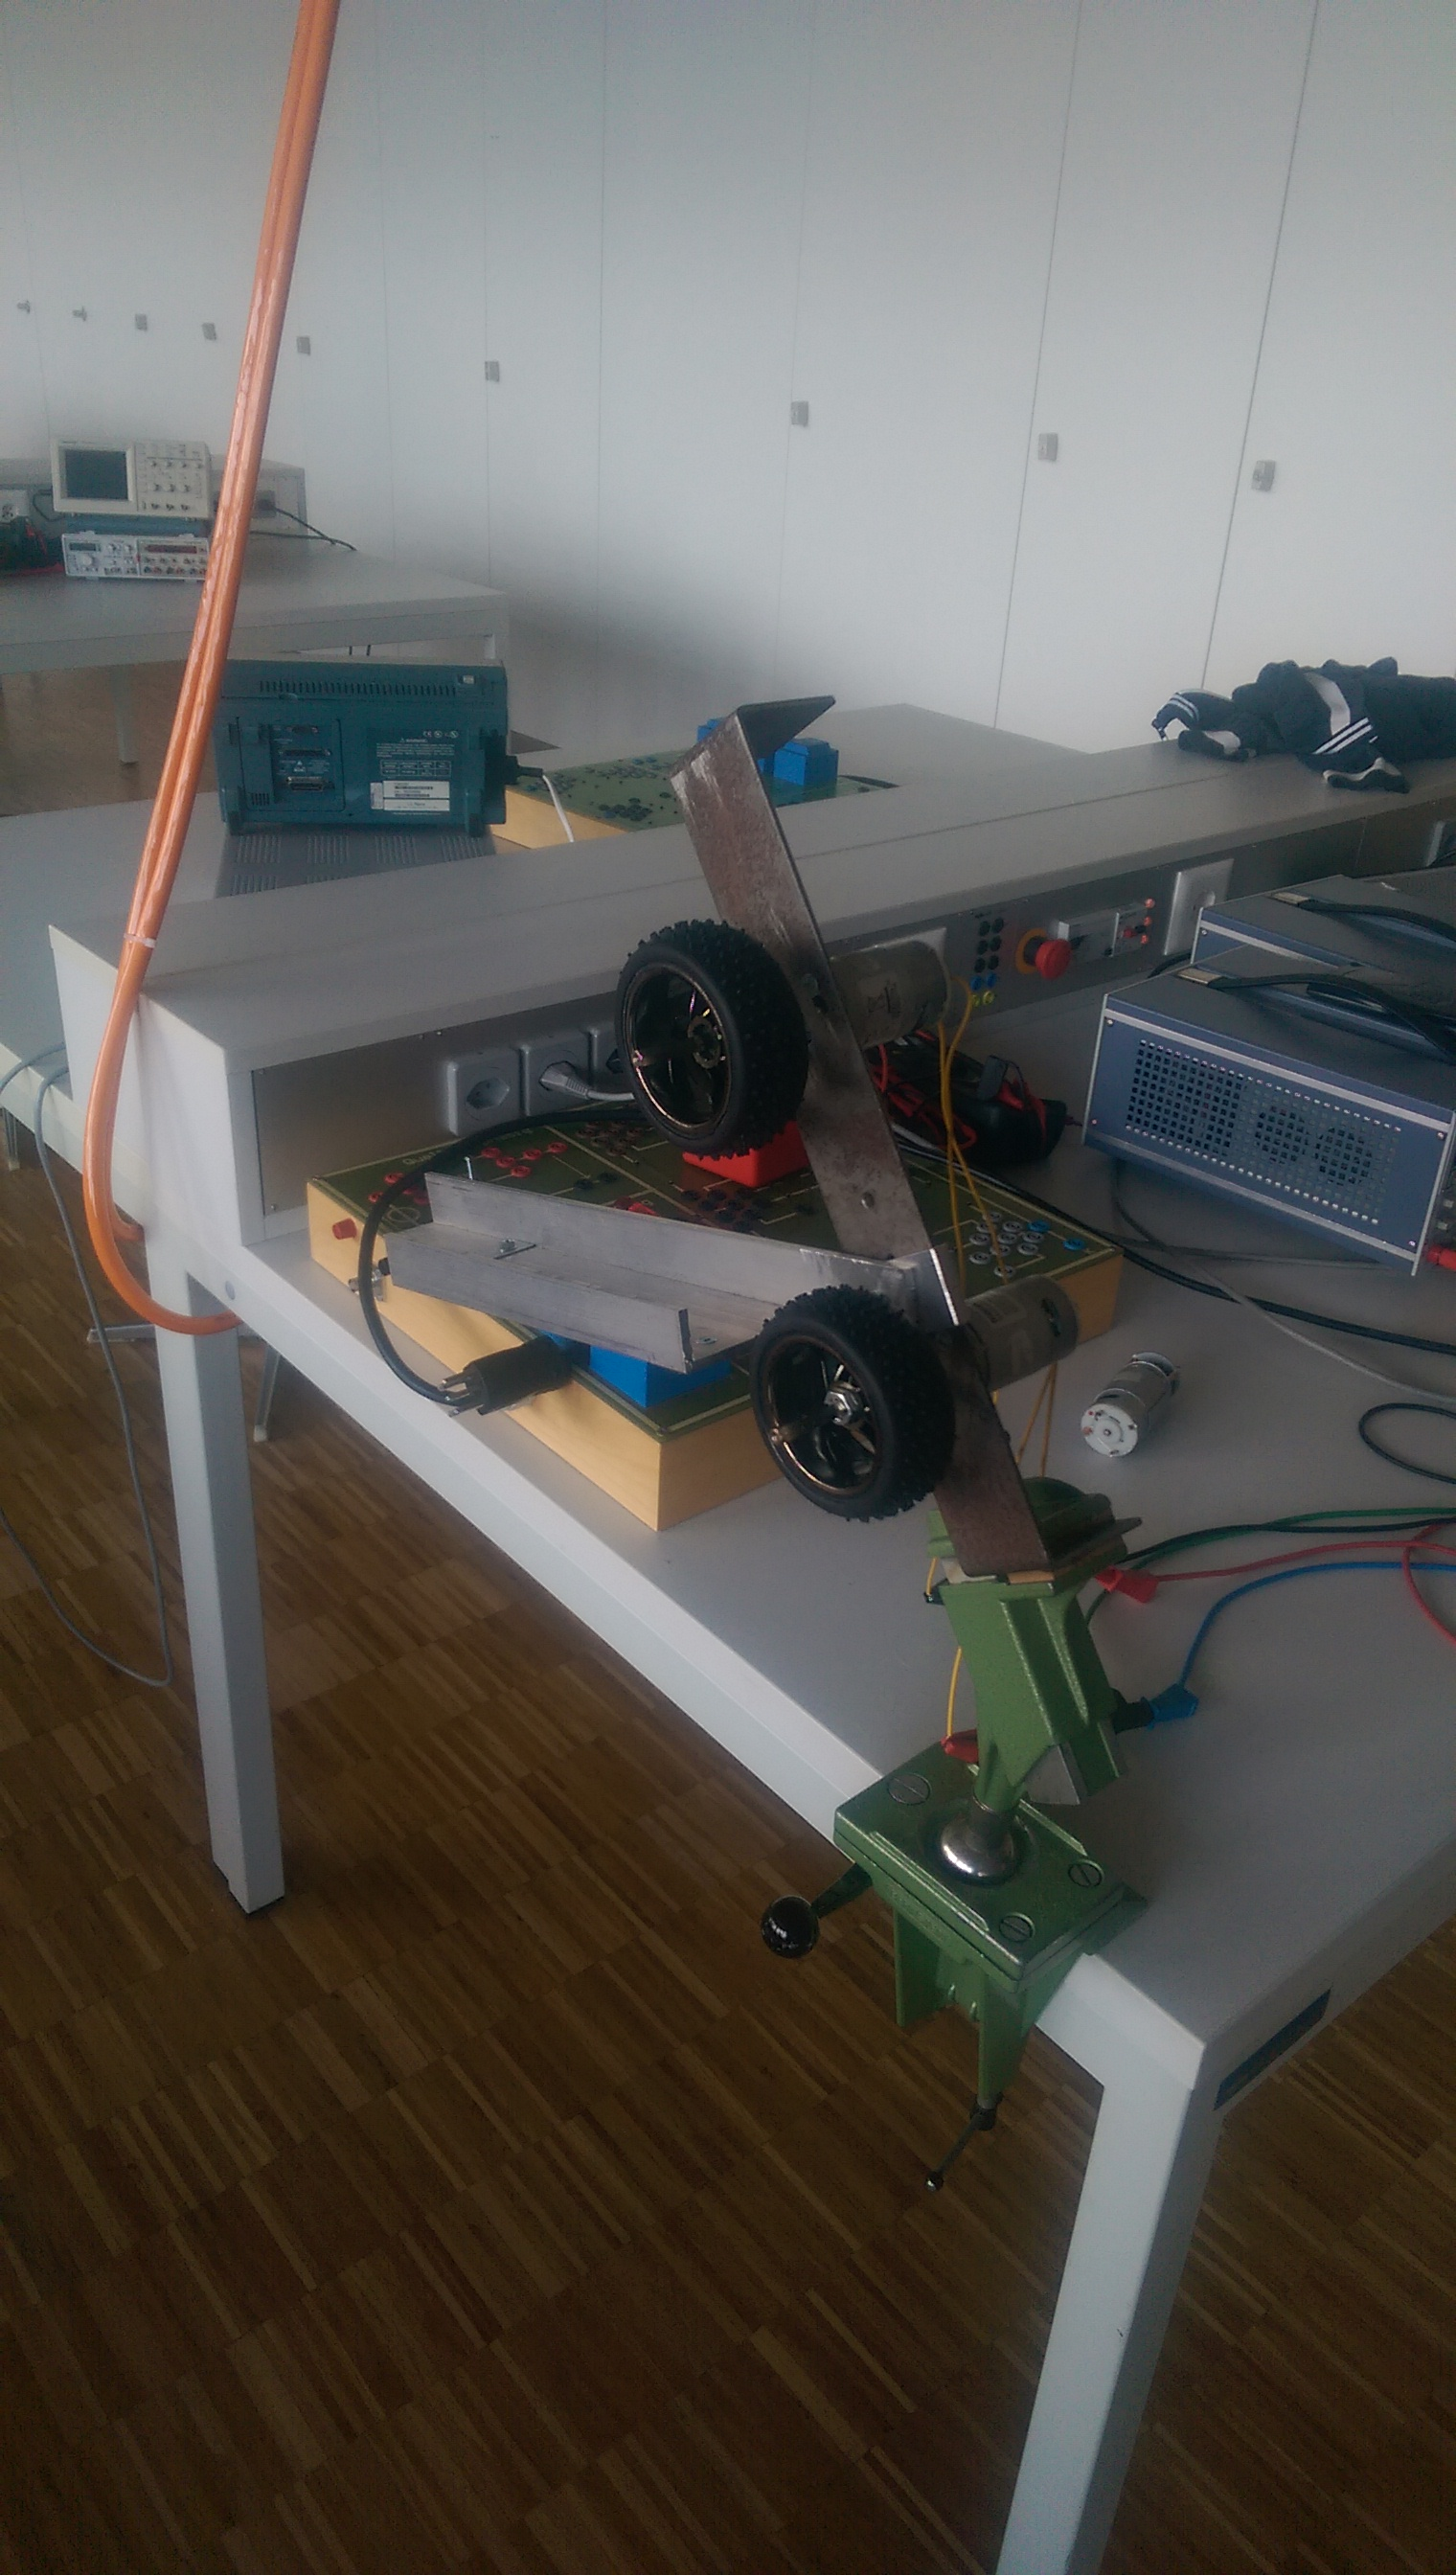
\includegraphics[width=0.7\textwidth,clip,trim=0mm 10cm 0mm 12cm]
	{Funktionstests/Bilder/Ballmaschine_Drehzahl1.jpg}
	\centering
	\caption{Funktionsmuster Ballmaschine} 
\label{abb:Ballmaschine_Drehzahl}
\end{figure}